There's a plethora of applications taking advantage of wearable tech, not all of them using the available bio sensors, ranging from basic real-time heart rate monitoring to progress tracking, to calorie measuring, and to social network sized fitness communities.

In this chapter I will research a few such applications and judge them based on following criteria:
\begin{itemize}
    \item Use of IoT possibilities -- use of available sensors, data collection from the community,
    \item User fitness assessment -- how the user's fitness is assessed (attempt self-assessment, fill out a questionnaire, or take a physical test),
    \item Community -- support of interaction between users,
    \item Extra features -- interesting perks that make the platform stand out among others,
    \item User-friendliness -- navigation around the mobile application - finding the general settings, creating and clearing a route, general user experience (the applications were tested on an Android phone),
    \item Availability -- the platform's economical model and its suitability,
    \item Cross-platform -- major operating systems supporting the mobile application and sensors, if any are used,
    \item Propriety -- whether the solution is open-source, closed-source or else.
\end{itemize}

%==============================================================================================
\section{komoot}
The cross-platform application for outdoor track suggestion can also be used as a tour planner, a map and a navigation system.

\subsection*{Use of IoT possibilities}
Given its use of GPS sensors, komoot does qualify as a basic IoT system, however, it also relies heavily on user input for route rating.
The smart watch only gets used for displaying of routes and navigation, not taking any advantage of the available biosensors.
\subsection*{User fitness assessment}
When a user is creating a route, they can set its difficulty as one of five levels, 
describing the user's self-reported physical fitness and their current will to take up a challenge (or lack thereof): \textit{Couch Potato}, \textit{Average}, \textit{In Good Shape}, \textit{Athletic}, and \textit{Pro}.
This parameter is considered when the app is generating a suitable route -- presumably by trying to adjust the elevation profile of the possible routes.
The user's real fitness is not taken into account.

\subsection*{Availability}
The region-based pricing model allows users who do not travel too much to use the app for free,
since the first region is provided at no cost.
In the other pricing options Single Region, Region Bundle and All Regions -- the price-performance ratio seems to grow at a reasonable scale.
\subsection*{Community}
With features like sharing and recommending of routes users have taken, following of other users, upvoting and commenting on their posts, the mobile application integrates a full-fledged social network.
\subsection*{Extra features}
Komoot supports multiple sports, mainly hiking, running and multiple types of biking, to which it tailors the parameters of planned routes, such as mostly paved roads for road bikes and gravel for off-road biking.
There are other activities the app supported by the app, which, however, do not offer the customized planning and can only be tagged later.
These sports include skateboarding, skiing, climbing, and plenty of others.
This only serves as a tag for the user with no real impact on the app's functionality.

If a user decides to skip all planning and just go into the world, their route can be ``recorded" for their use or the use of other komoot users, who can pick this route and either

\begin{enumerate}[label=\alph*)]
    \item follow it `as is', with all the possible deviations from the known network of streets and paths with the risk of impassable roads, or
    \item have komoot replan the off-grid segments and navigate through the known street network, or
    \item edit the route according to one's liking.
\end{enumerate}

Users can pick a starting point, a destination, as well as any number of waypoints in between for their route (see fig.\ref{komoot-nav-img})
Once the route is chosen, the user can go through the route's stats - the estimated time it will take to get from start to finish, its length, the elevation profile (see fig.\ref{komoot-route-details-img}, \ref{komoot-route-elevation-detail-img}) (uphill, downhill, highest and lowest points, estimated average speed) and the surfaces and their use in proportion to the route's length (see fig.\ref{komoot-route-surface-overview-img}).
All this information is delivered in easy-to-understand charts as well as interactive mappings -- using a slider, the user can see which stat applies to which part of the route.

\begin{figure}[h!]
    \centering
        \tmpframe{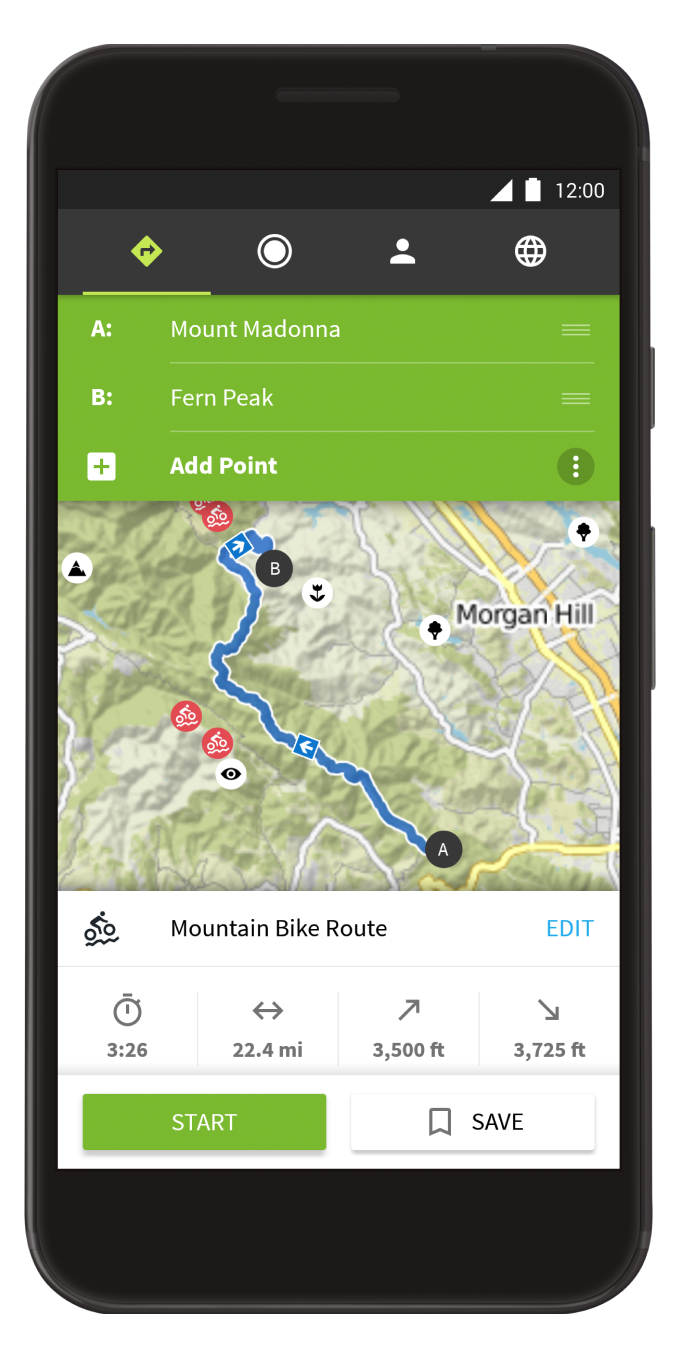
\includegraphics[width=0.4\textwidth]{Images/komoot-nav.png}}
        \caption{Route planning in the komoot app~\cite{komoot-nav-img}.}
        \label{komoot-nav-img}
\end{figure}

\begin{figure}[h!]
    \centering
        \tmpframe{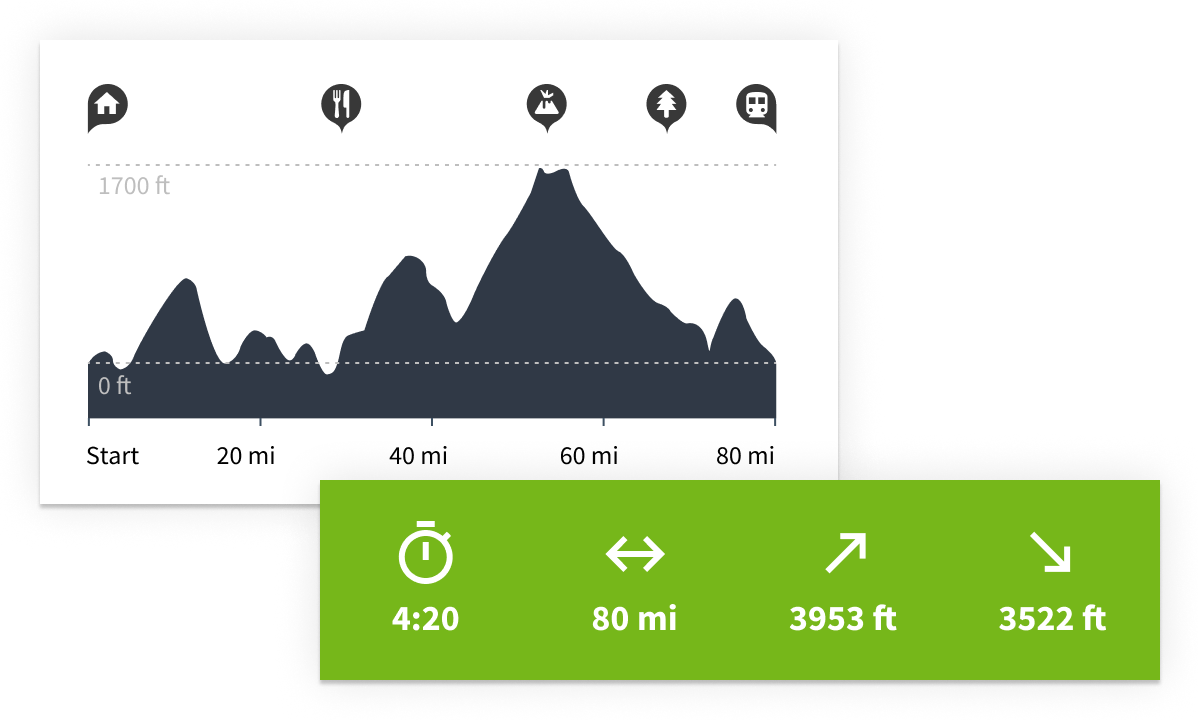
\includegraphics[width=0.8\textwidth]{Images/komoot-route-details.png}}
        \caption{Route elevation profile~\cite{komoot-route-details-img}.}
        \label{komoot-route-details-img}
\end{figure}

\subsection*{User-friendliness}
The mobile app uses a bottom tab bar for navigation, however, the way the tabs are designed is not entirely user-friendly.
The \code{Plan} and \code{Record} tabs are clear enough, but the \code{Profile} tab contains a lot of information that does not seem entirely connected to the user's profile, such as people to follow and the app's settings.
The last tab, titled \code{More}, only contains promotions for komoot offline maps and komoot premium, which is something a user does not expect under this tab.
The navigation through the mobile app takes some time to get used to -- it took me a while to find the Settings after I did not see them in the \code{More}menu on the bottom tab bar.

Once I created a route, the information provided was well-delivered and easy to read, however, there was no obvious way of completely cancelling the chosen route and picking another one.
Instead, hiding in the Options of the route -- which I had not noticed before -- I found the "Reset route" option, which cleared the route.
Overall, the app makers made some great UX decisions, but also some that do not seem natural to the user.
\subsection*{Cross-platform}
The system is fully integrated with the Apple Watch and Samsung gear, and -- at least limitedly -- supports a number of other brands of smart watches and other Bluetooth-enabled devices.
The mobile application runs both on iPhones and Android phones.
\subsection*{Propriety}
The system is not entirely open-source, as a few of their repositories are public, but the core components remain proprietary~\cite{komoot-github}.

\begin{figure}[h!]%
    \centering
        \subfig
        \tmpframe{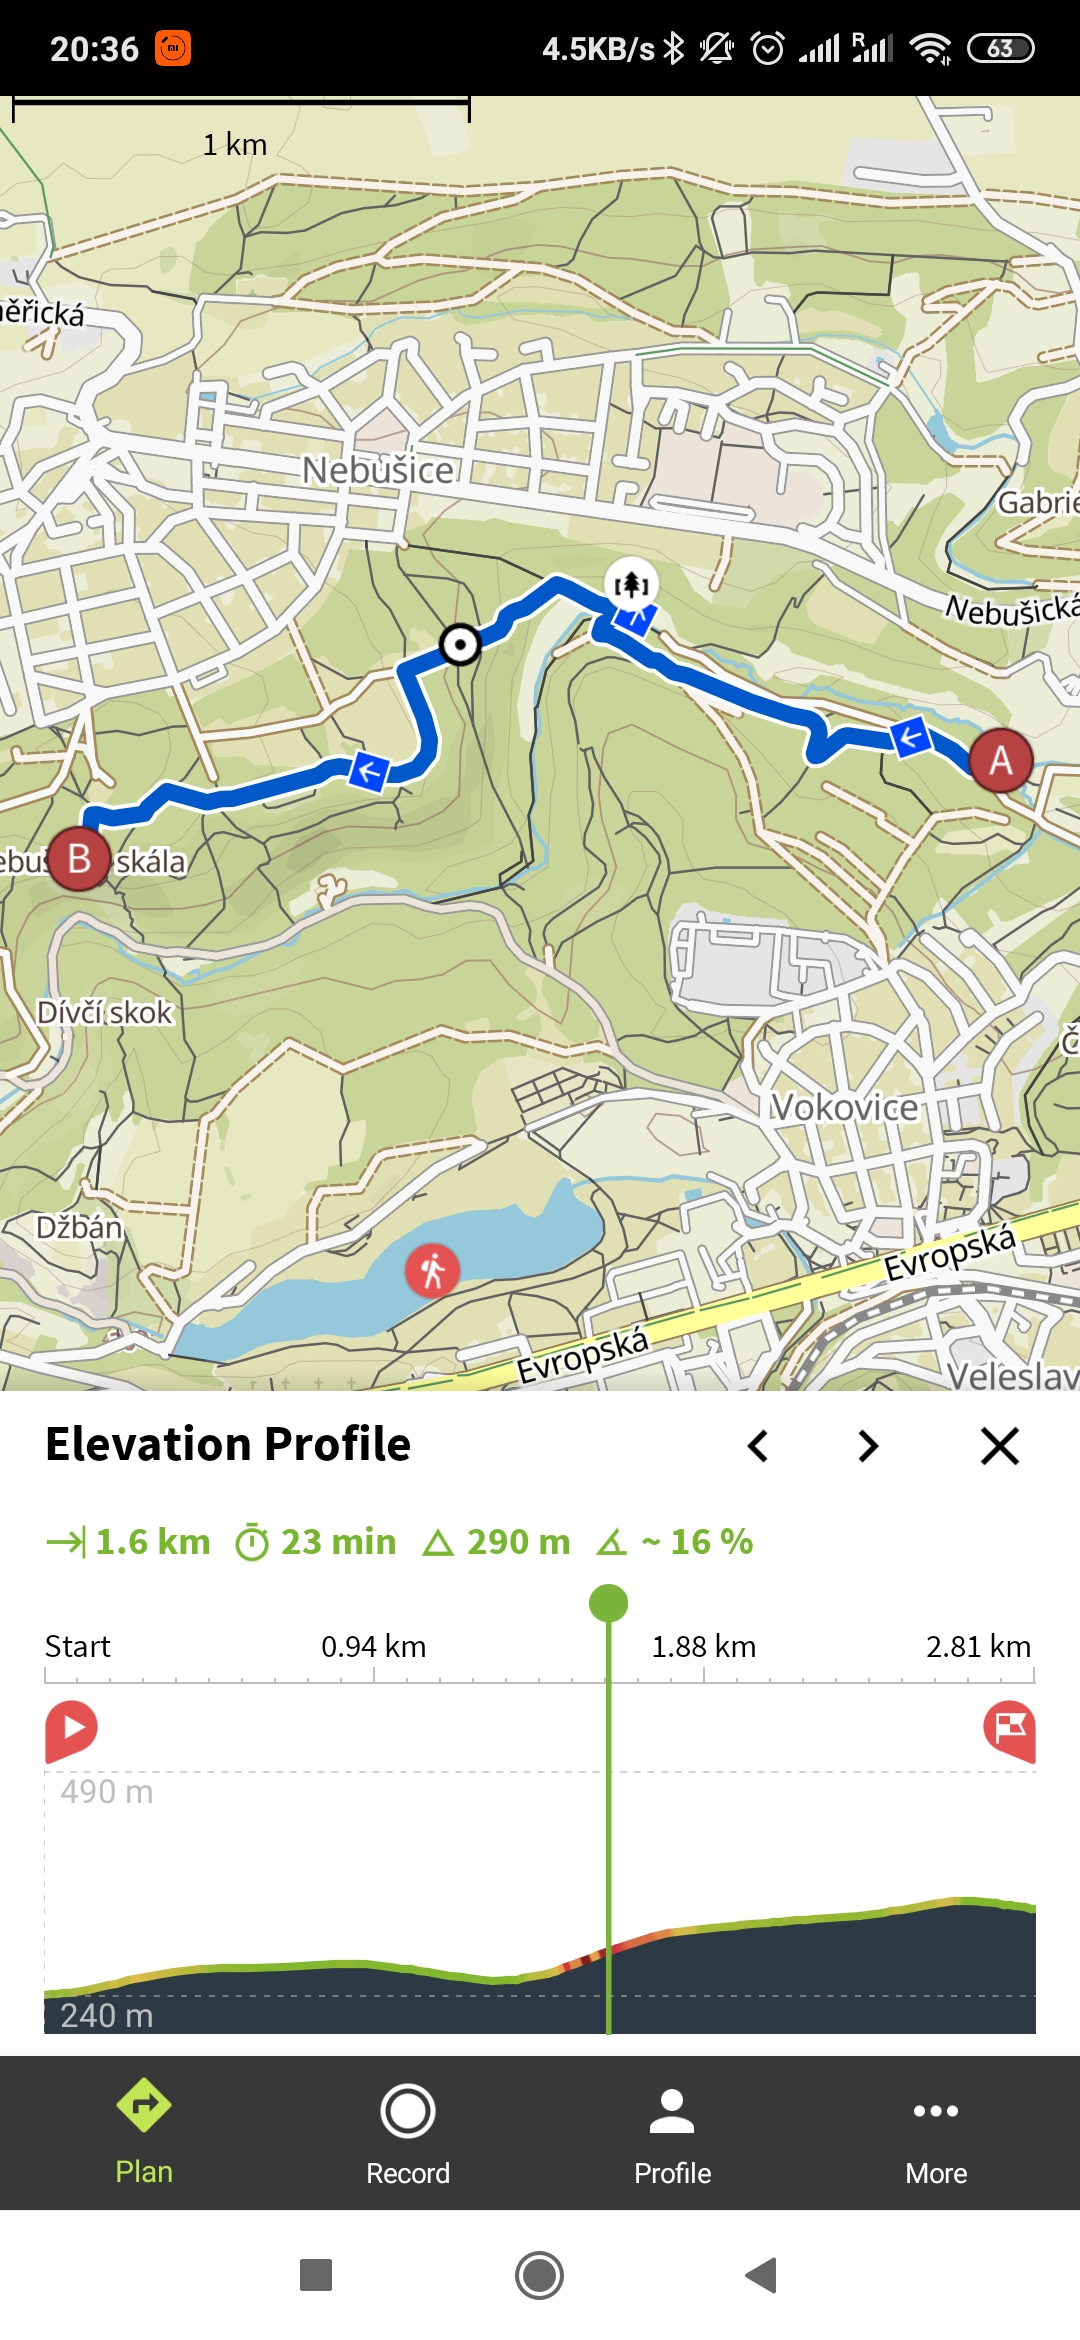
\includegraphics[width=0.4\textwidth]{Images/komoot-route-elevation-detail.jpg}}
        \caption{Overview of the route's elevation~\cite{komoot-route-elevation-detail-img}.}
        \label{komoot-route-elevation-detail-img}
\end{figure}
\begin{figure}
    \centering
        \tmpframe{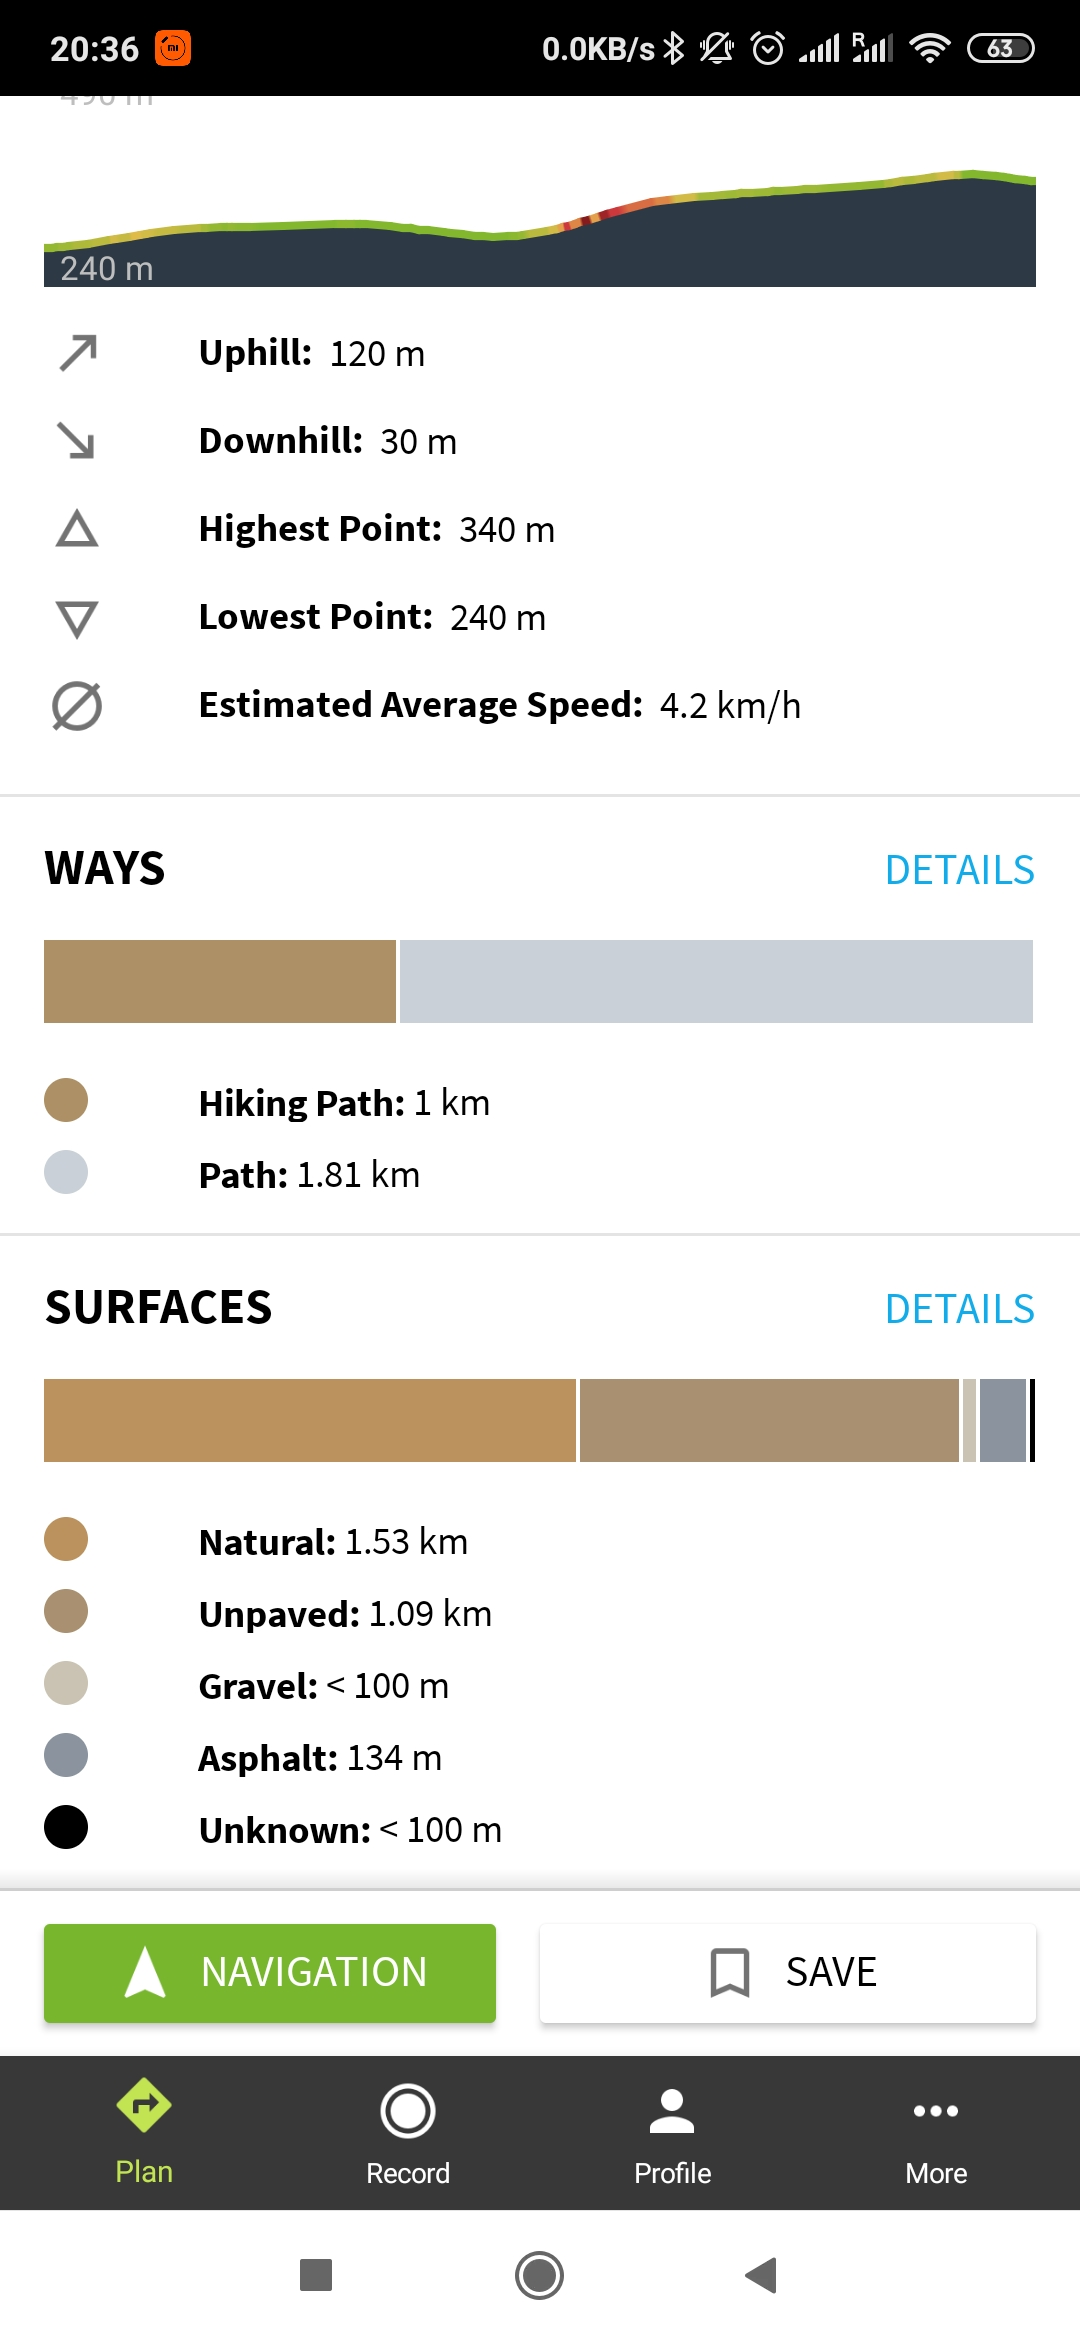
\includegraphics[width=0.4\textwidth]{Images/komoot-route-surface-detail.jpg}}
        \caption{Overview of the route's surface~\cite{komoot-route-surface-overview-img}.}
        \label{komoot-route-surface-overview-img}
\end{figure}

%==============================================================================================
\pagebreak
\section{endomondo}

Under Armour's endomondo application serves as a personal trainer for distance-based sports, such as running, cycling, or hiking.
Their main focus is on the endorphin release people get from encouragement and motivation -- this is why the app gives coaching advice, allows the users to send each other peptalks, and has over the course of its existence built a global fitness community.
\subsection*{Use of IoT possibilities}
The application integrates with a wide range of watches and sensors, collecting data from GPS trackers, bicycle speed and cadence sensors, bike power sensors and heart rate measurement units.
Some basic statistics based on this data (such as average heart rate) is presented to the user with a free plan, 
while the more interesting statistics displayed with interactive graphs are for premium users only -- average heart rate history, heart rate zone analysis, even weather information collected from AccuWeather.com at the time of the workout.

The application used to have a feature called Peer Banchmark, which used other users' data to compare the user with the rest of the community, however, this feature was removed due to lack of use~\cite{endomondo-HR-max-emails}.
\subsection*{User fitness assessment}
The premium version of the application promises personal exercise plans for running goals, and the heart rate zones are calculated using the Karvonen formula: 
\[((max HR − resting HR) × \% Intensity) + resting HR\]
However, endomondo's website does not mention how and when HRmax and HRmin are calculated, and the official support personnel does not have any additional information about what is written on their website~\cite{endomondo-HR-max-emails}.
In spite of that, the values for the Karvonen formula are pre-filled when a user accesses the page, so they probably use age-based formulas to estimate all the variables.
In any case, they are all editable, so if the user already knows their HRmax for example from a laboratory test, they can use it.
When creating a new training plan (that is, having endomondo calculate the ``ideal'' plan for how a person should train if they want to run a specific distance on a specific day in the future),
one of the steps has the user choose a recent workout which will be used for calculating the individual's fitness level and for the plan generation~\cite{endomondo-training-plan-fitness-assessment}.
\subsection*{Availability}
Endomondo comes in two versions -- free and premium.
The free version has basic functionality, which is so limited that some have opted for free alternatives with more useful features such as Strava or Runmeter~\cite{endomondo-review}.
It is supported by not too obtrusive ads on the bottom of the screen.

The premium version is ad-free, brings a number of necessary features such as heart rate zones, training plans, and others, and is based on a monthly subscription.
\subsection*{Community}
Endomondo's main focus in keeping their users on the platform is motivation, which is also demonstrated by the application's slogan -- ``Free your endorphines''.
One of their features is a real-time audio motivator, which makes comments on how well the user is doing compared to previous workouts,
encouraging them if they are lagging behind or is informing them about the personal record they are be about to hit.

Competing against oneself, however, is not as much fun -- and therefore as motivating -- as getting to beat a friend or relative at the activity of choice.
This is why the application also integrates a social network of millions of users with functions like sharing one's activities, sending peptalks and challenges.
\subsection*{Extra features}
After the end of the workout, you can answer a ``How was your workout?'', however, since this is a plain text option, this data is only for the user's later reading, and cannot be used in any machine processing.

A user can post photos in the description of the activity, as well as use tags which are useful on social media after sharing.
With premium, one can filter based on these tags -- useful for tracking the number of kilometres that the user has run in a specific pair of shoes, or biked with a specific chain.
Other users can also be tagged, for example running partners or the person you are trying to beat in a challenge.

The premium version of the app also includes a few modes for interval training (periods of exercise alternating with periods of normal-to-high intensity training) as well as the option to build your own.
There are many applications that support this feature -- after all, it is just fairly basic time tracking -- but it is nice to have all the functionality in a single app.
\subsection*{User-friendliness}
The navigation in the mobile application is realized with a bottom tab bar, whose design is nicely done.
The \code{More} tab hides a lot of functionality, effectively serving as an easy-to-reach hamburger menu.

Given the fact that that endomondo does not support planning of routes and merely follows where the user is headed, the \code{Workout} tab which contains a map is less crowded than in a navigation app (fig.\ref{endomondo-home-img}).

\begin{figure}[h!]
    \centering
        \tmpframe{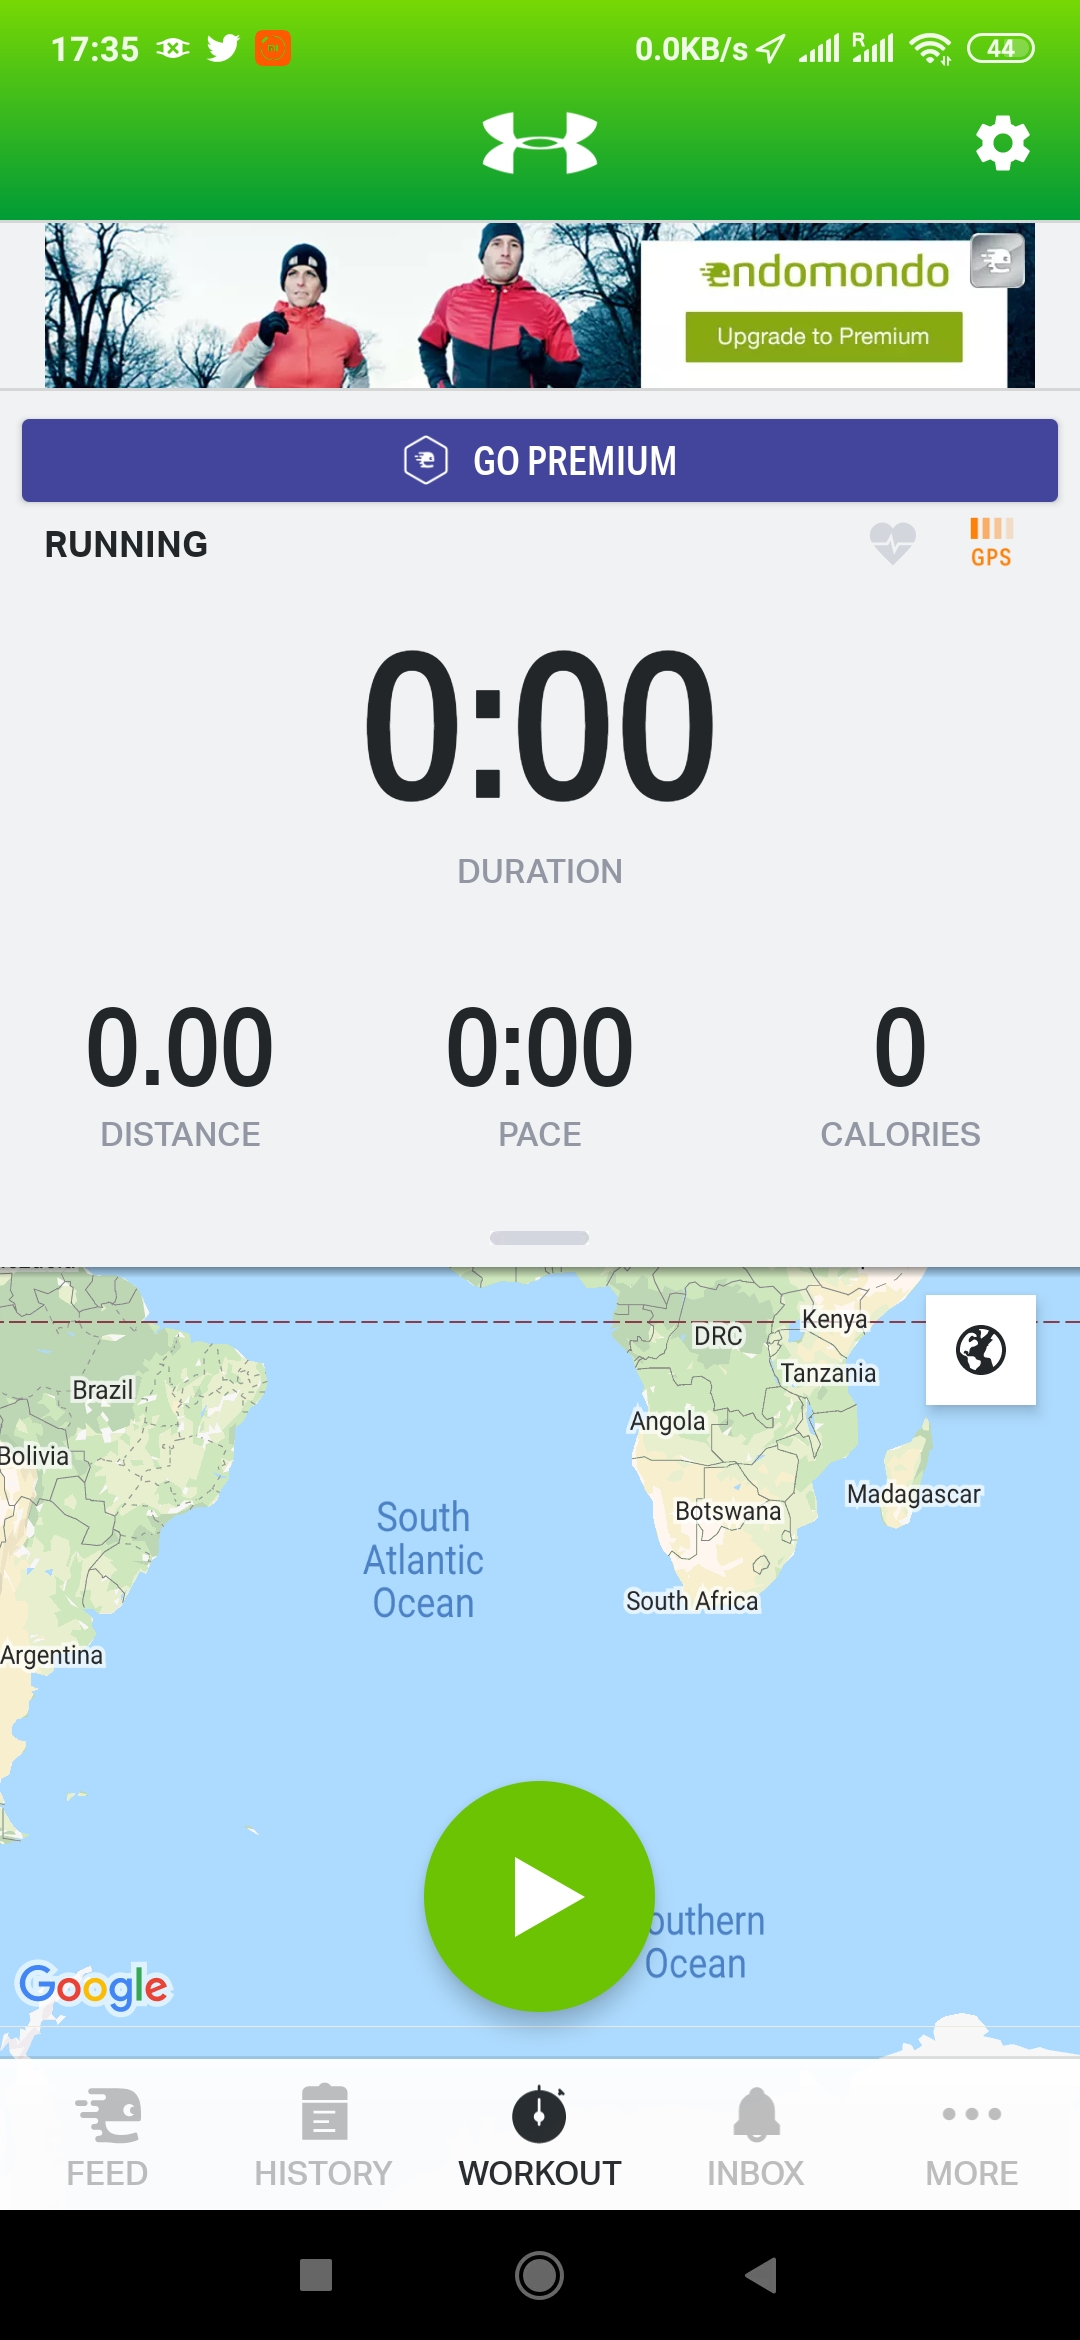
\includegraphics[width=0.4\textwidth]{Images/endomondo_home.jpg}}
        \caption{endomondo's main screen~\cite{endomondo-home-img}.}
        \label{endomondo-home-img}
\end{figure}

The main settings can immediately be found in the top-right corner of the main screen, or under the \code{More} tab, lost in between ten other options (fig.\ref{endomondo-more-tab}).
The application is easy to navigate and is fully made in, if somewhat blocky-feeling, material design.


\begin{figure}[htb!]
    \centering
        \tmpframe{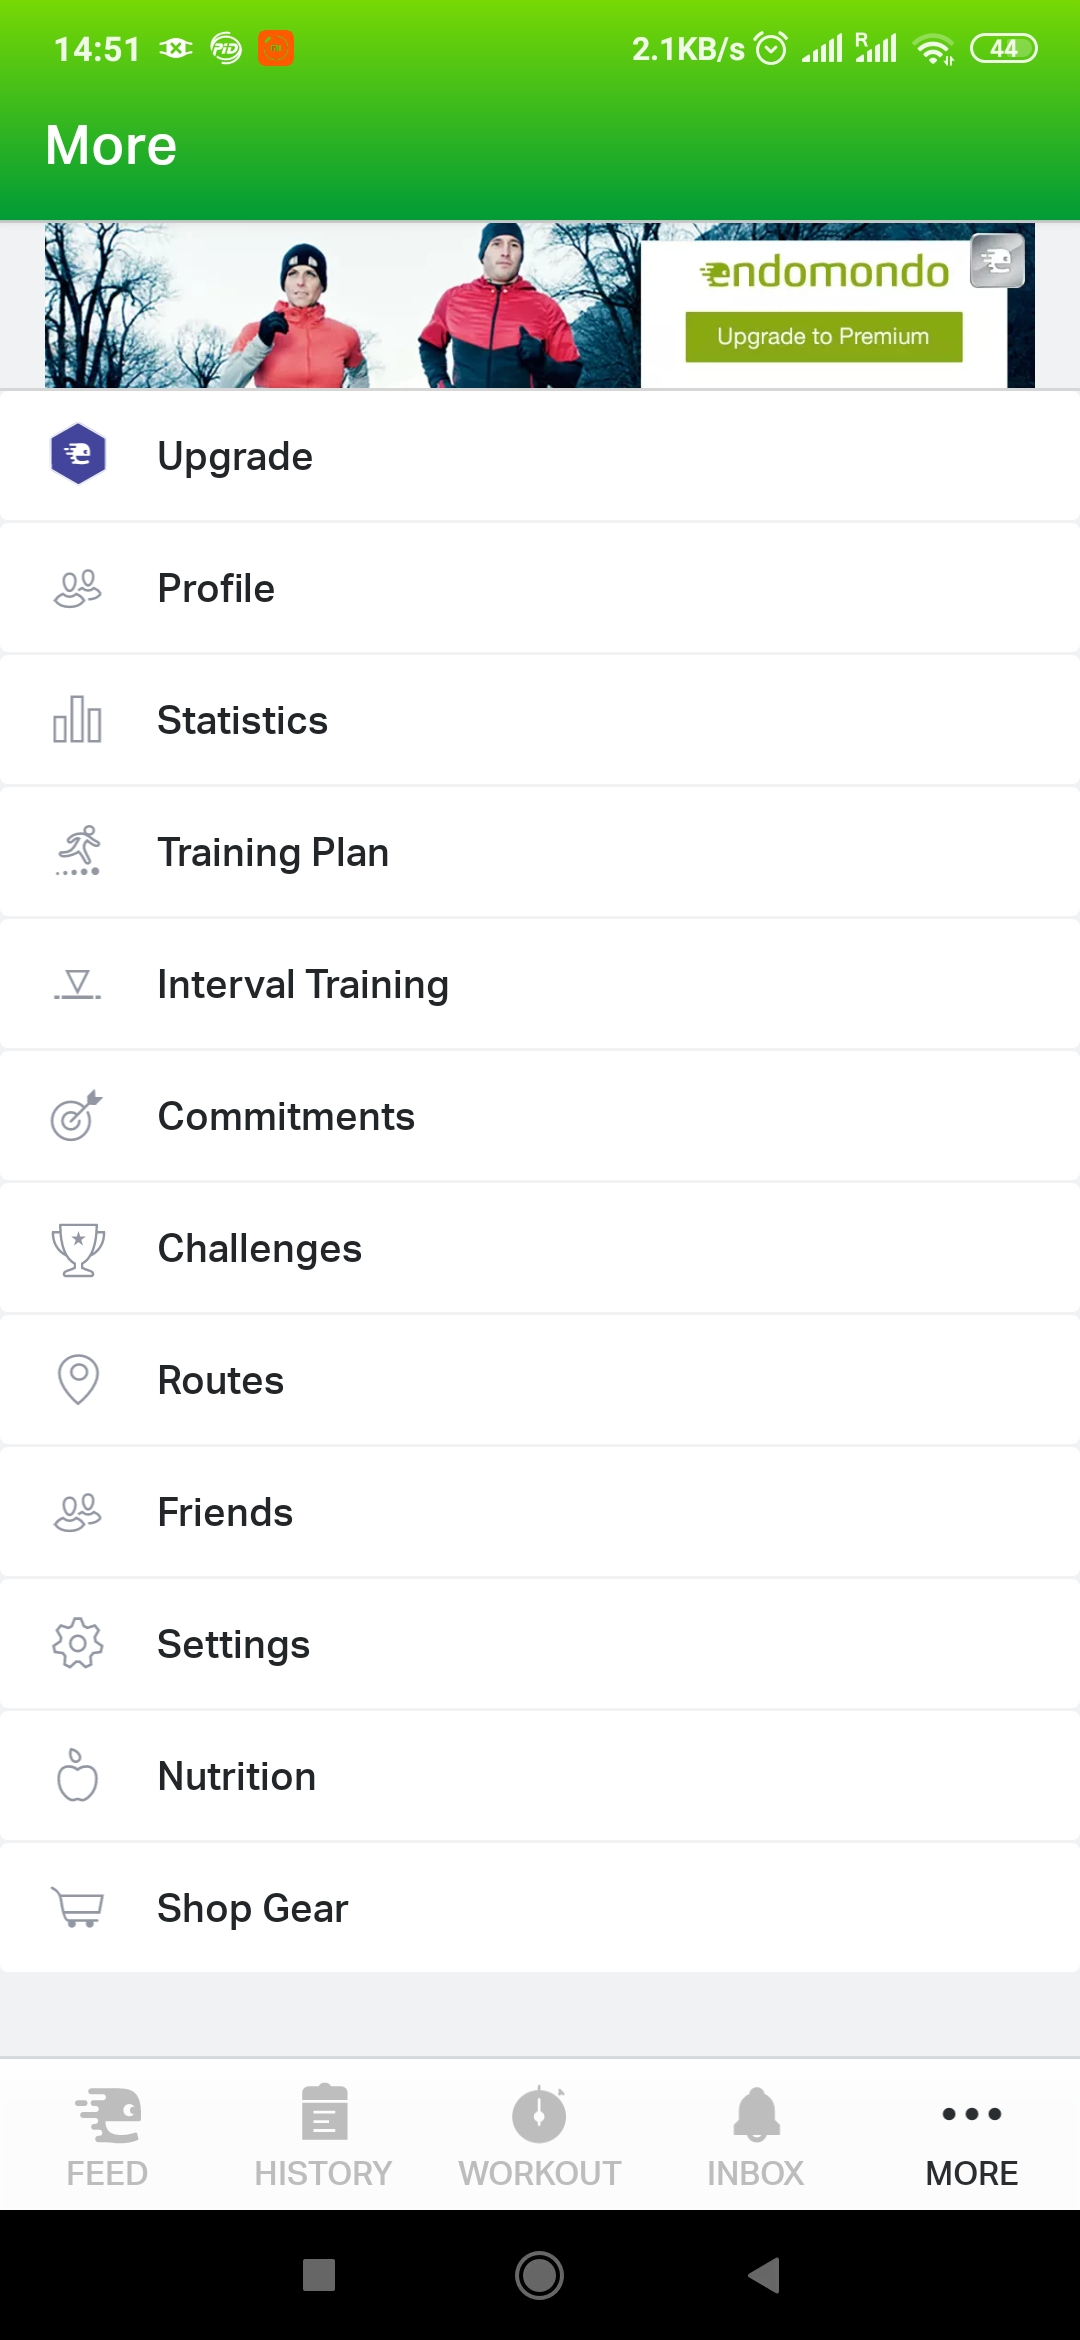
\includegraphics[width=0.4\textwidth]{Images/endomondo-more-tab.jpg}}
        \caption{endomondo's \code{More} tab, with main settings lost in other options~\cite{endomondo-more-tab}.}
        \label{endomondo-more-tab}
\end{figure}

\begin{figure}[htb!]
    \centering
        \tmpframe{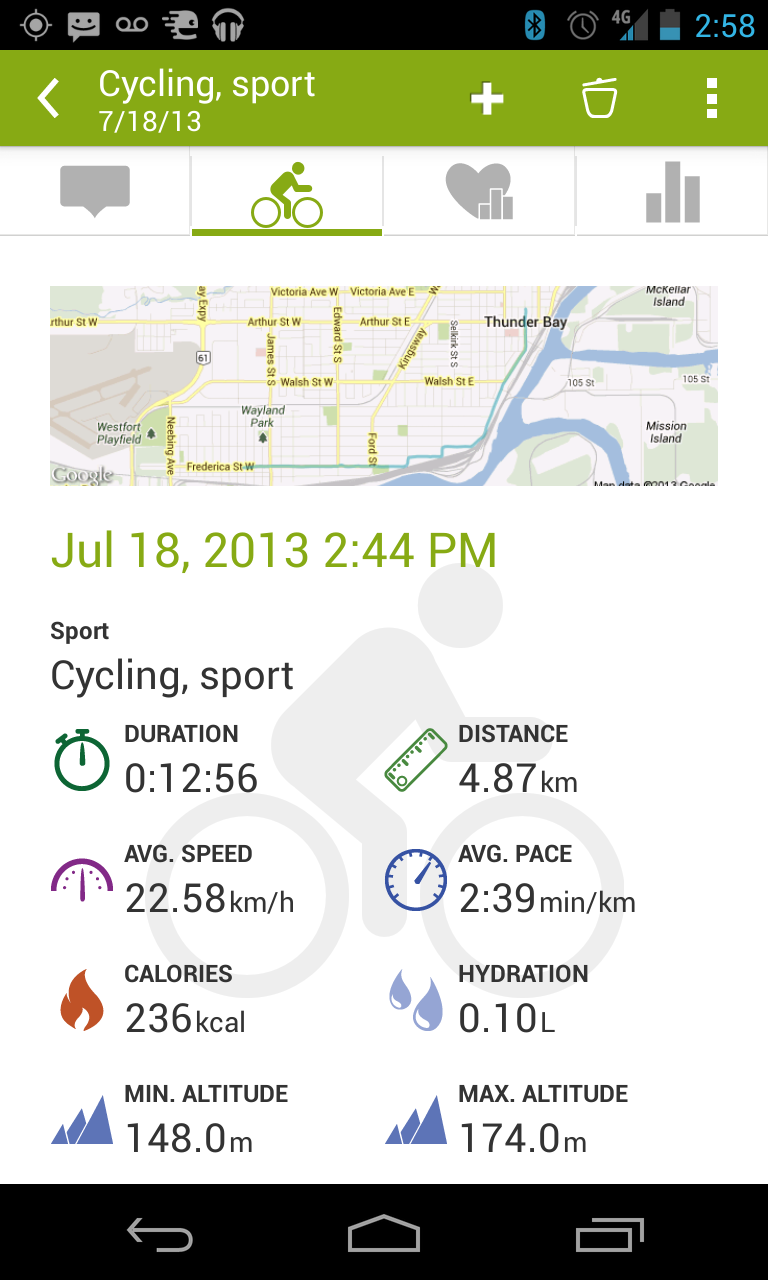
\includegraphics[width=0.4\textwidth]{Images/endomondo-bike-stats.png}}
        \caption{Statistics of a biking trip on endomondo~\cite{endomondo-bike-stats-img}.}
\end{figure}

\begin{figure}[htb!]
    \centering
        \tmpframe{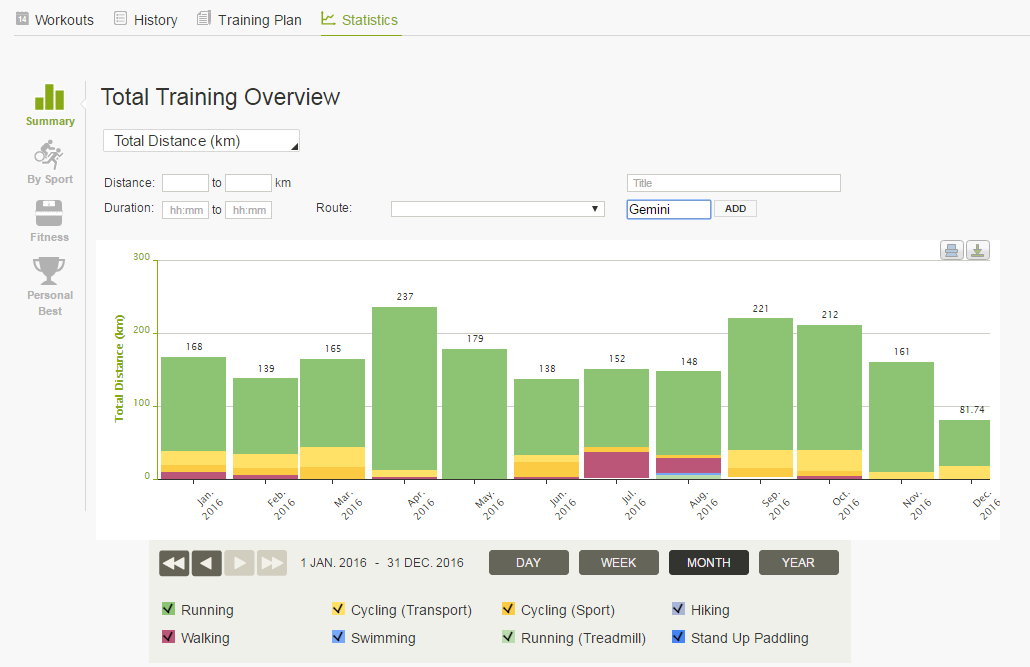
\includegraphics[width=\textwidth]{Images/endomondo-history-example.png}}
        \caption{endomondo history example from the web application~\cite{endomondo-history-img}.}
\end{figure}

\subsection*{Cross-platform}
All the features are available for iOS 9 and newer and Android 4.1 and newer.
Endomondo also used to be available on Blackberry and Windows phones.
Some features are only available in the web application.
\subsection*{Propriety}
The whole endomondo application only has a single public repository on github, which is a fork of tapiriik -- a tool for data synchronization between different fitness applications, such as Endomondo, Garmin Connect, Strava, Runkeeper, and others~\cite{endomondo-tapiriik}.
Otherwise, the whole application is completely proprietary.
%==============================================================================================
\pagebreak
\pagebreak
\section{Strava}
Strava is a social network for athletes that offers a large number of features mainly focused on tracking and analysis of users' activities, sharing, and competing~\cite{strava}.
The target sports of the platform are running and cycling, but it supports plenty of other activities.
It has both a web and a mobile application, with some features shared and some only available in one of them.
\subsection*{Use of IoT possibilities}
Strava makes good use of sensors in the users' devices -- those for measuring heart rate, power, and GPS.
The platform creates heatmaps of routes that are used the most, taking advantage of their tracking technology and the users' GPS sensors.
They also use a novel way of determining the surface of routes, thanks to data not only from OpenStreetMap, but also from the users' bicycle frames.

\subsection*{User fitness assessment}
The Strava platform includes plenty of user fitness-related components, such as the premium \code{Fitness \& Freshness} feature,
which shows the user how fit they are on a graph of past activities, and how fresh, based on the amount of exercise the user has recently done,
all of this calculated using power data and heart rate or perceived exertion~\cite{strava-fitness-freshness}.
The platform also has heart rate zones, which are primarily calculated using an age formula, but the user can manually customize them.
\subsection*{Availability}
Strava is available both for free and for an affordable monthly subscription.
\subsection*{Community}
The platform has millions of active users who are connected in a large social network.
It allows users to create clubs, such as groups of friends as well as racing teams.
These clubs give the user the opportunity to keep track of the members' activity and exercise, with feeds and leaderboards.

For increased safety while outside, Strava Beacon is a premium feature that allows a user's friend to see their real-time location in case of an emergency.

Another community-building perk is the feed of challenges (fig.\ref{strava-challenges}), which help motivate the users with leaderboards and competitiveness.

\begin{figure}[h]
    \centering
    \tmpframe{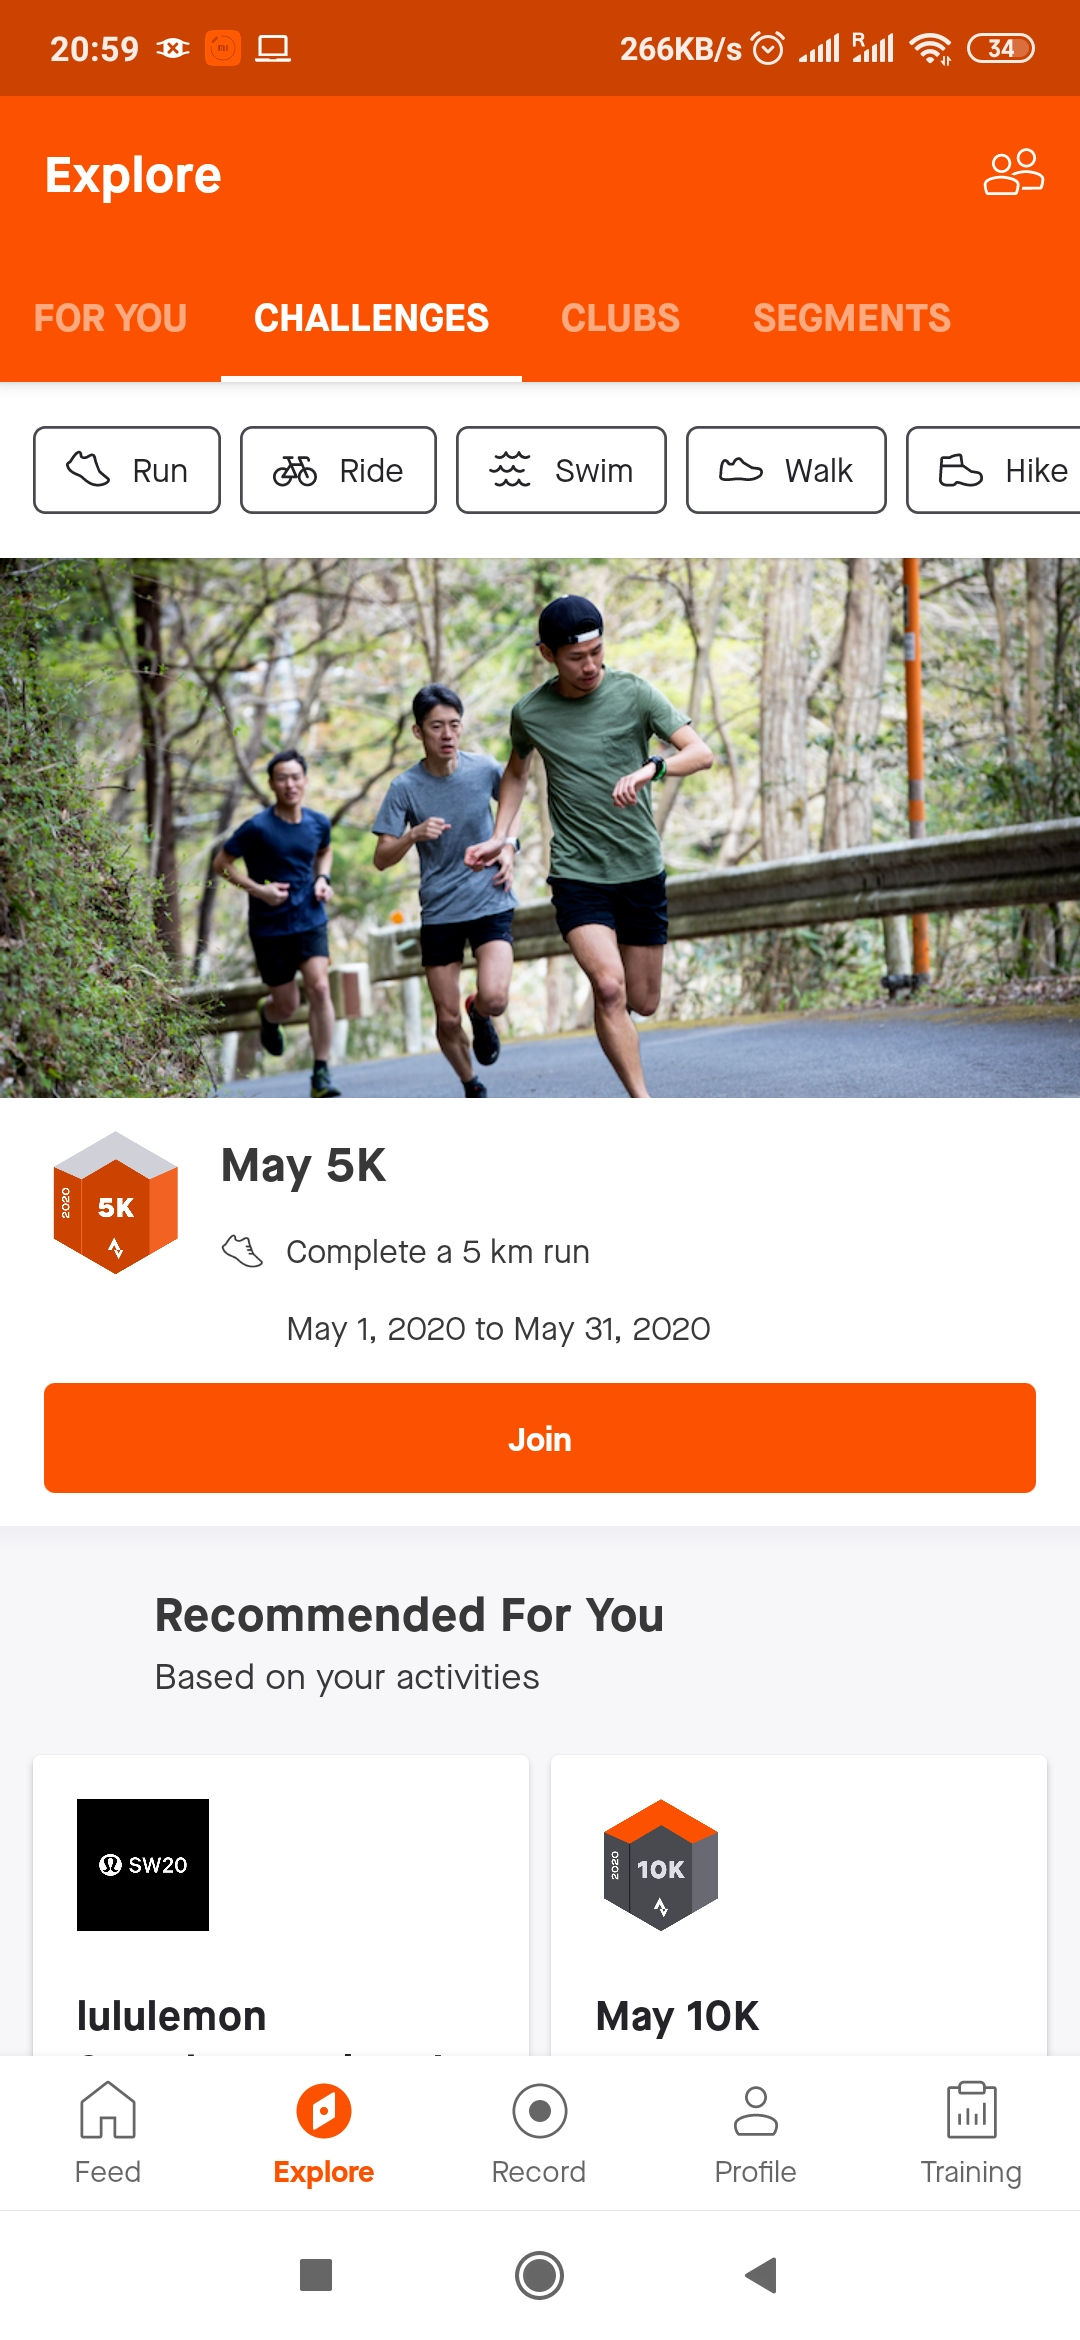
\includegraphics[width=0.4\textwidth]{Images/strava-challenges.jpg}}
    \caption{Challenges feed on Strava~\cite{strava-challenges}.}
    \label{strava-challenges}
\end{figure}

\subsection*{Extra features}
One of the most popular premium features is called Segments (fig.\ref{strava-segments-img}), where users can compare their times on specific portions of road or trail using leaderboards.
This is supported by heatmaps of use frequency of specific routes.
It also allows the user to input their pictures, gear, and perceived exertion to the activity session.
The premium version of the platform offers a lot of features that are somewhat less connected to fitness but make it successful as a social network.

\begin{figure}[htb!]
    \centering
        \tmpframe{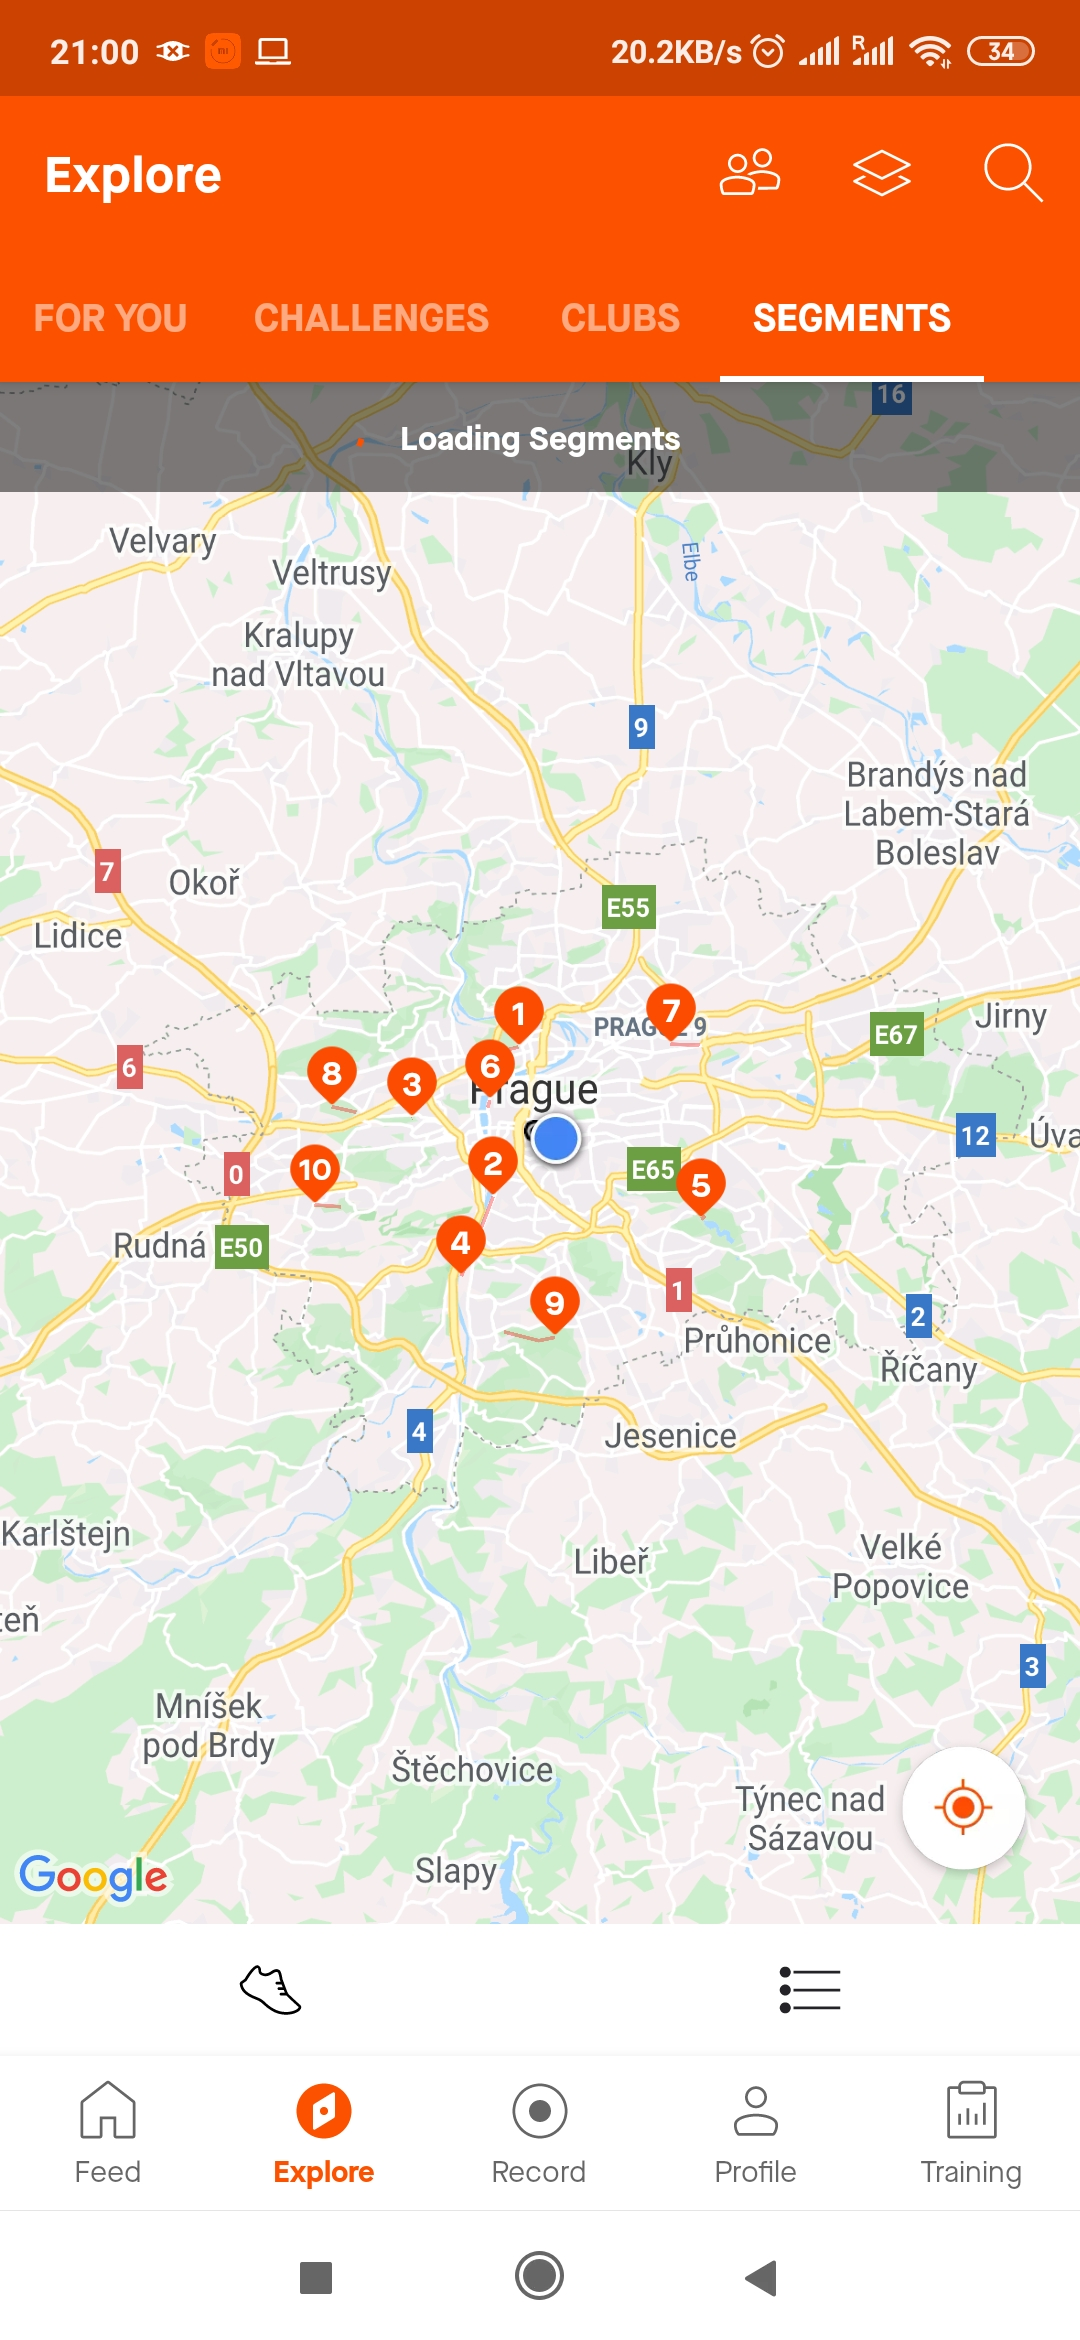
\includegraphics[width=0.4\textwidth]{Images/strava-segments.jpg}}
        \caption{Strava segments near the user's location~\cite{strava-segments-img}.}
        \label{strava-segments-img}
\end{figure}

\subsection*{User-friendliness}
The mobile app uses a tab bar for navigation, with nicely thought out tabs - \code{Feed} tab for posts from the community, \code{Explore} tab for challenges, clubs, and segments,
the central \code{Record} tab for the actual activity, which is simple and clutter-free, with the options to change the sport, pick a route, and turn on the Strava Beacon.
Another tab \code{Profile} keeps the user's account details and fitness information, such as their stats, activities, and training log.
The last tab \code{Training} contains the user's training plans, which are part of the premium subscription.

One thing that I missed was the option to create a route on the phone -- this can only be done in the web app and then synchronized with the mobile app, making the mobile application less suitable for ad hoc navigation.

Another unusual design decision was putting the \code{Find friends} button only on some pages.

\begin{figure}[h]
    \centering
    \tmpframe{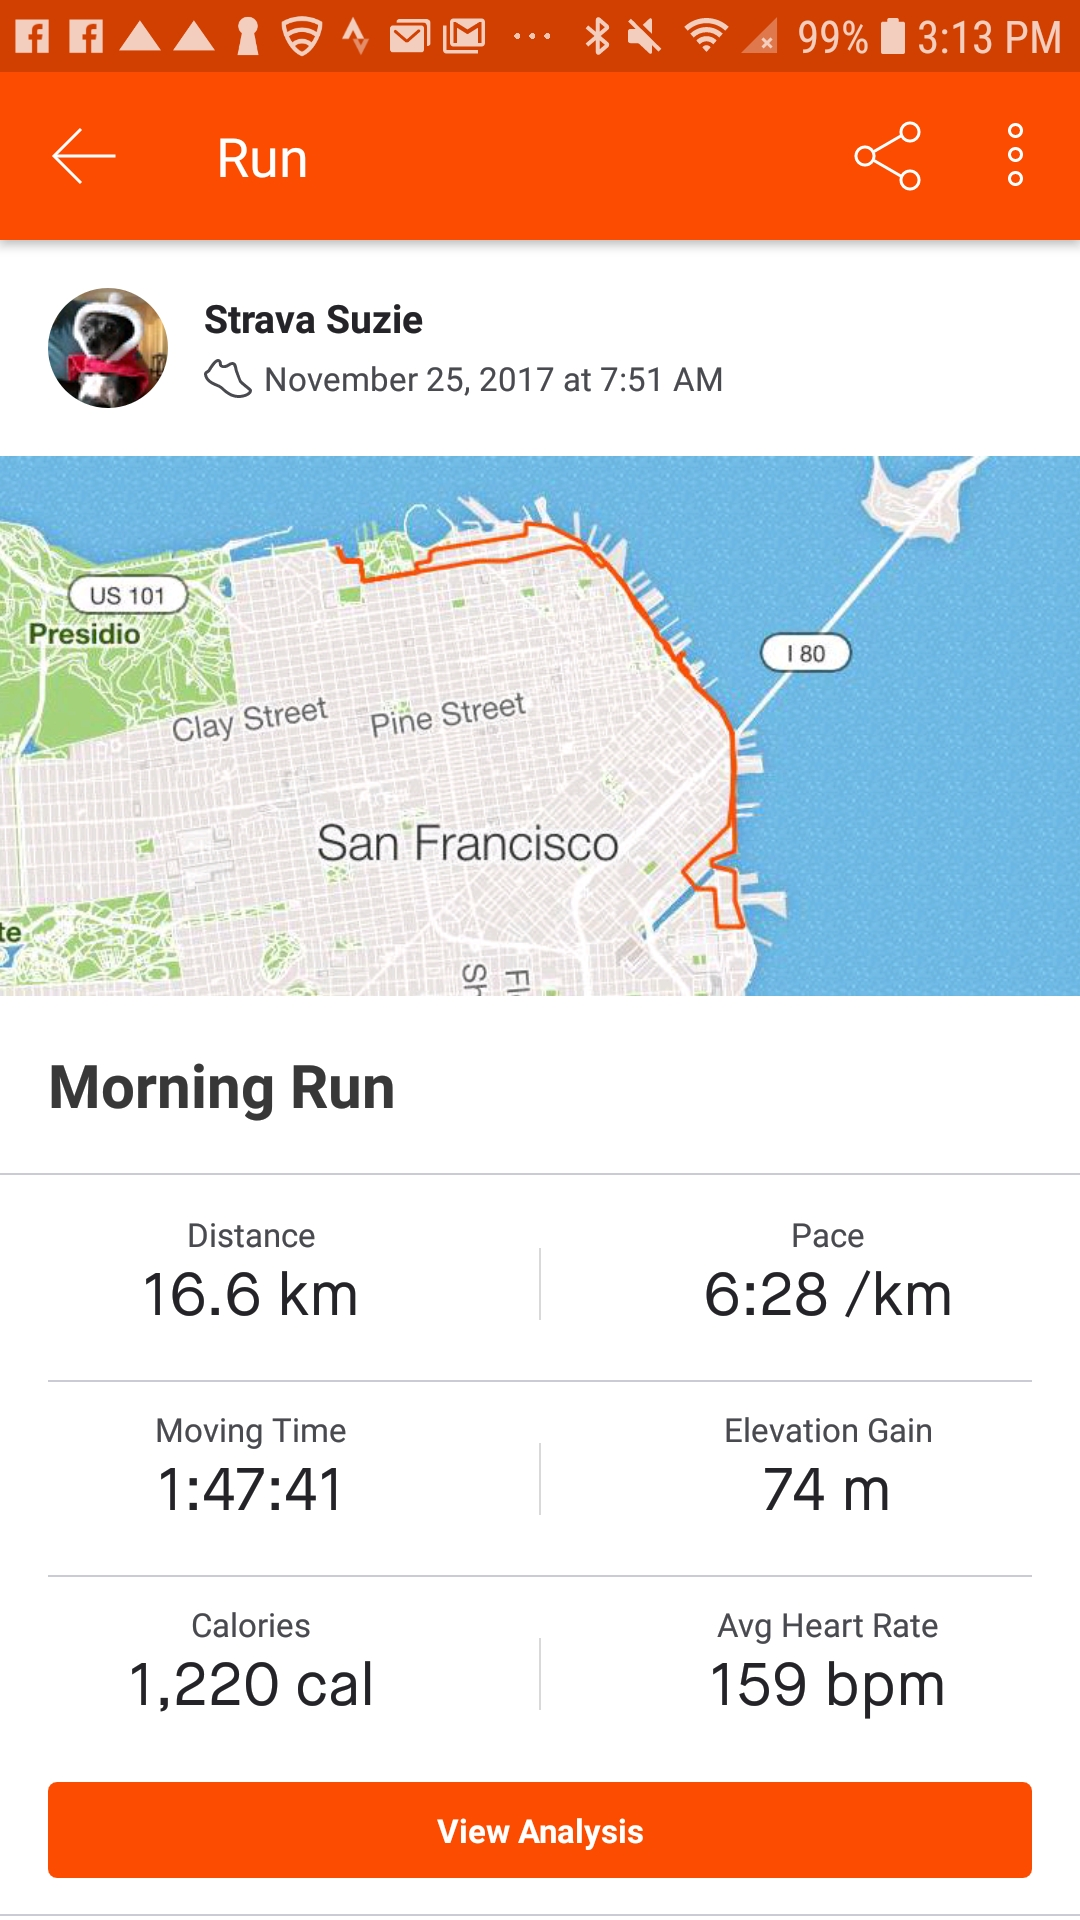
\includegraphics[width=0.4\textwidth]{Images/strava-morning-run-stats.jpg}}
    \caption{Statistics of a run on Strava~\cite{strava-run-stats-img}.}
    \label{strava-run-stats-img}
\end{figure}

\subsection*{Cross-platform}
The mobile app Strava is available both on Android and iOS, as well as providing a web application.
It supports a variety of smart watches, power sensors, and other devices.
\subsection*{Propriety}
The application is closed-source, but it offers a publicly available API for custom development.
%==============================================================================================
\section{Garmin Explore and Garmin Connect}
The vast ecosystem Garmin has created for their users is filled with an assortment of wearables, radars, smart lights, navigations, customized maps, and plenty more, providing features which are presented to the user via modular mobile apps.

Here I will analyse the Garmin Explore application, which is targeted at hikers, in tandem with Garmin Connect, which functions as a fitness tracker.

\subsection*{Use of IoT possibilities}
Most fitness-focused Garmin watches do have a heart rate sensor and all of them include a step counter, however, this data is never compared with that of other users, keeping focus on the user's activity history with no prediction.
The Garmin Connect app includes an ``Insights'' feature, which compares the user's simpler data, such as daily number of steps or hours of sleep, to that of all other users.
\subsection*{User fitness assessment}
Some of the heart-rate-monitor enabled watches allow a user to set the zones (see chapter on fitness assessment) in which they would like to keep their heart rate depending on the activity they choose to do.
The Connect app also allows users to manually input their VO2 max, but doesn't test the user on it.

As mentioned in the Fitness assessment chapter, they offer the Performance condition stat, which however, according to user feedback, isn't useful or accurate.

\begin{figure}[h]
    \centering
        \tmpframe{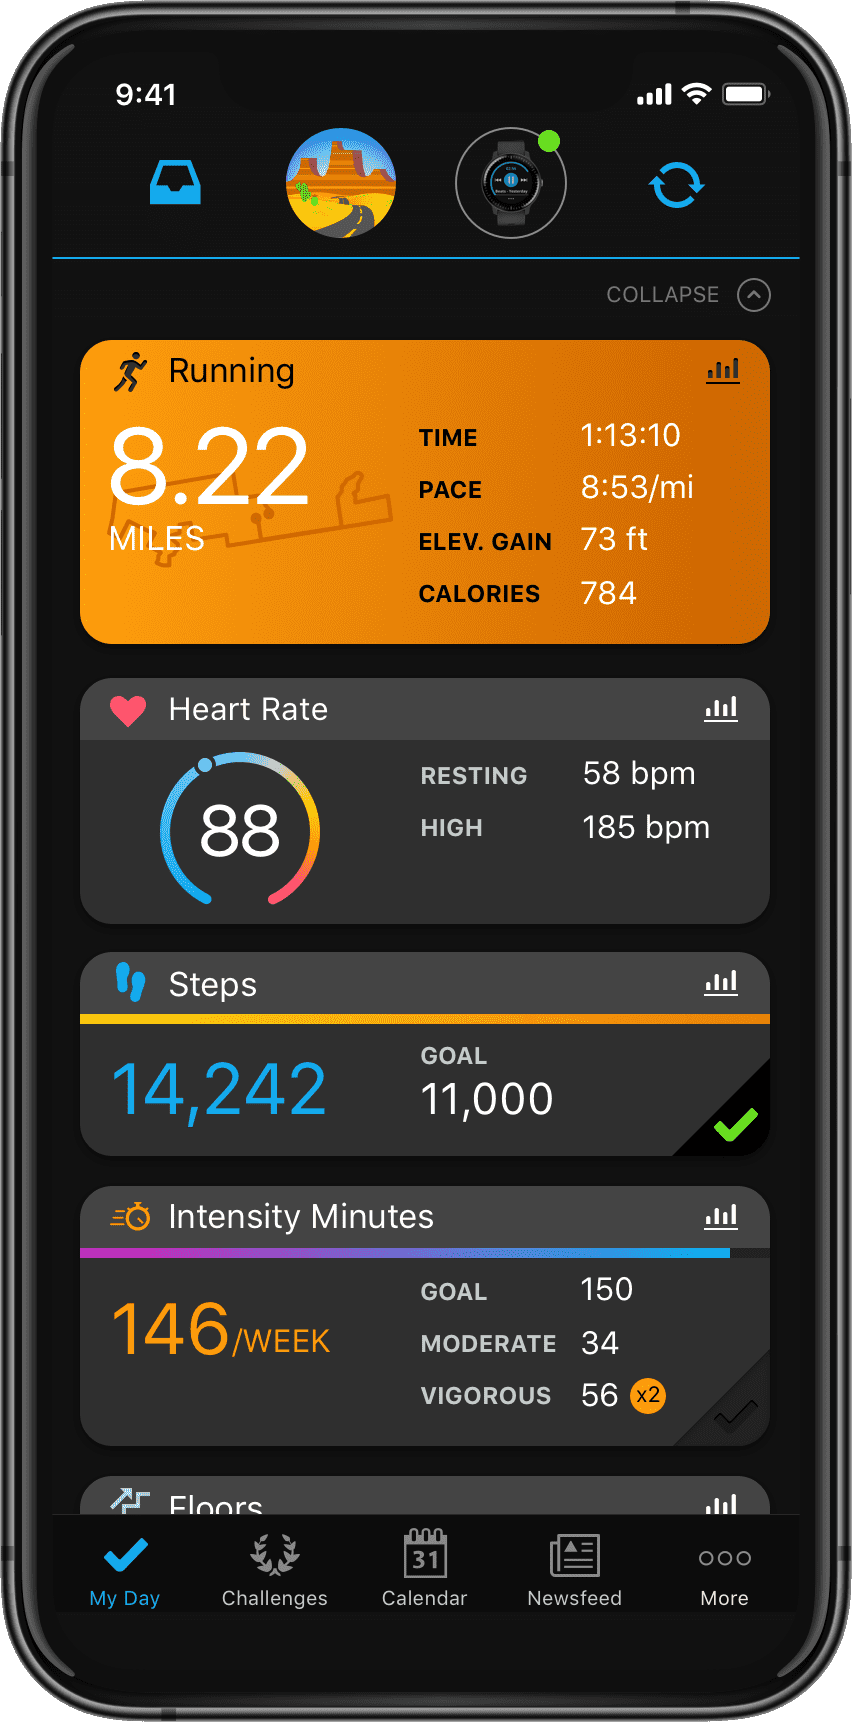
\includegraphics[width=0.4\textwidth]{Images/garmin-connect-myday-screen.png}}
        \caption{My day - Garmin Connect's home screen displays statistics of the user's recent activity~\cite{garmin-my-day-img}.}
        \label{garmin-my-day-img}
\end{figure}

\subsection*{Availability}
In general, Garmin's pricing model relies on the user buying one of their high-end smartwatches, whereupon the rest of the components (apps, basic maps, support, etc.) are free, with some exceptions, such as advanced maps. 
The company's smartwatches are considered premium quality, with a wide price range - target groups include \textit{potential Rolex buyers}~\cite{garmin-expensive} as well as ordinary users~\cite{garmin-watches-review}.
\subsection*{Community}
The Connect application handles the data from the point of view of a fitness tracker, with social features like groups, competitions, likes, comments, and badges of accomplishment~\cite{garmin-connect}.
\subsection*{Extra features}
The Explore application is very simple, mostly just containing the bare necessities such as the map, route planning, and a history of activities.
It doesn't even contain navigation options; it is hard for me as a user to understand what its use is.
It allows the user to group waypoints, tracks, routes and activities into collections for each trip.
The Connect application, as a fitness tracker, gives insights into the user's fitness, allows to track the lifespan of the user's gear, their sleep quality, water intake, menstrual cycle (as this can affect the user's stamina), and other factorss.
\subsection*{User-friendliness}
The modularity of Garmin's apps allows for cleaner, easier-to-navigate interfaces.

The Garmin Explore app uses a tab bar for navigation; and while the four tabs do not have any inscriptions, the icons manage to communicate fairly clearly what the user can find in them.
In the Map tab, it took me a while to find the button for creating a new route or waypoint (top-left corner in fig.\ref{fig:garmin-map}), since it does not stand out from the other UI components.
The actual track creation process feels natural, visual and light-weight, with fast waypoint creation and editing, however, I lacked the option to search for a place that I would want to use as a waypoint.
A large disappointment for me as a user was the fact that I did not get a planned route -- only the polyline defined by the waypoints, which seems completely useless for navigation purposes.
Once the route was saved and shown on the map, I could not figure out how to cancel it.

\begin{figure}[h]
    \centering
        \tmpframe{\includegraphics[width=0.4\textwidth]{Images/Garmin-map-tab.jpg}}\hfill
        \tmpframe{\includegraphics[width=0.4\textwidth]{Images/Garmin-route-create.jpg}}
        \caption{Garmin's map tab~\cite{garmin-map-tab-img} and route creation screen~\cite{garmin-route-create}.}
        \label{fig:garmin-map}
\end{figure}

Another interesting decision is the Library tab, which contains the user's past activities, saved waypoints, routes, and tracks.
The difference between the (otherwise synonymic) words ``route'' and ``track'' is that a route is the generated polyline, whereas a track is a set of breadcrumbs of a past hike.

The Connect app, as the main fitness app in the Garmin ecosystem, entails a larger number of features, resulting in a full tab bar as well as a hamburger menu, which I found a little confusing.

\subsection*{Cross-platform}
All of Garmin's applications can be installed both on Android and iPhone.
However, they can only be paired with watches inside Garmin's ecosystem, which is a drawback for users who already own a smartwatch.
\subsection*{Propriety}
Some of the Garmin applications are completely open-source, either due to the software that they are derived from, or simply to provide the general public with opportunity to customize their Garmin experience~\cite{garmin-open-source}~\cite{garmin-connect-github-repos}.
These apps are mostly concerned with map handling, navigation and sound codecs, but also include some bits of functionality like widgets, low power watch apps and others.

While some of this code may be used in the Explore or Connect applications, these repositories don't contain their core functionality.

\section{Summary}
All of the studied platforms are used by a wide community of users, are either mostly or completely closed-source, base their maps off the OpenStreetMap, and have their own ways (or lack thereof) of integrating IoT principles in their design.

Komoot is a great app for navigation; its flexible way of route planning gives the user a good idea of what they can expect on their trip,
and includes navigation.
However, the information provided is not tailored to the user's actual fitness level.

Endomondo tracks the user's progress and motivates them.
Since there is no route planning, it doesn't estimate the difficulty of outdoor tracks -- instead it serves as a personal trainer.

Strava is great at tracking and analysing data from previous activity, and at providing new ways for athletes to connect and motivate each other.
It gives the user a good insight into their data, and allows comparison between users on pre-defined segments.
But again, there are no estimations done or tests to be taken.

Garmin Connect is a great fitness tracker, but the Explore app is not useful for route planning or navigation.

None of the apps fully customize their assessment of the user's fitness to estimate how they will do on their future hikes, which is a core feature of my application.

There is an abundance of community features in all of these apps; it is reasonable to consider how many of them are enough to keep the users entertained and how many become overwhelming.

